\documentclass[]{article}
\usepackage[utf8]{inputenc} 
\usepackage[T1]{fontenc}
\usepackage[upright]{fourier} 
%\usepackage[usenames,dvipsnames]{xcolor}
\usepackage{tkz-kiviat} 
\usetikzlibrary{arrows}

\usepackage{pgfplots}
%\usepackage{tikz}



\thispagestyle{empty}  

\begin{document} 

\begin{tikzpicture}[label distance=.15cm,rotate=30,scale=.65]
\tkzKiviatDiagram[radial=7,lattice=4,gap=1,step=0.2,label space=2]%
       {Maths,
        Histoire Géo,
        Français,
        EPS,
        SVT,
        Techno,
        Physique}
  \tkzKiviatLine[thick,color=red](6.5,5,7.5,1,2.5,5, 15)
  \tkzKiviatLine[thick,color=blue](15,16,13,18,11,7, 18)
  \tkzKiviatGrad[prefix=,unity=5](0)   
 \end{tikzpicture}


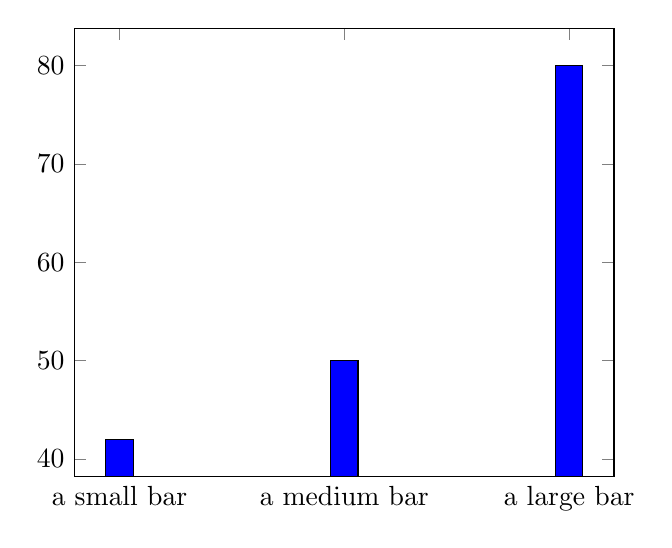
\begin{tikzpicture}
\begin{axis}[
symbolic x coords={a small bar,a medium bar,a large bar},
xtick=data]
\addplot[ybar,fill=blue] coordinates {
	(a small bar,42)
	(a medium bar,50)
	(a large bar,80)
};
\end{axis}
\end{tikzpicture}

%	\begin{	tikzpicture	}
%		\begin{	axis}[
%			ybar,
%			enlargelimits=0.15,
%			legend style={at={(0.5,-0.15)},
%				anchor=north,
%				legend columns=-1},
%			ylabel={\#participants},
%			symbolic x coords={tool8,tool9,tool10},
%			xtick=data,
%			nodes near coords,
%			nodes near coords align={vertical},
%			]
%			
%			\addplot coordinates {(tool8,7) (tool9,9) (tool10,4)};
%			\addplot coordinates {(tool8,4) (tool9,4) (tool10,4)};
%			\addplot coordinates {(tool8,1) (tool9,1) (tool10,1)};
%			\legend{used,understood,not understood}
%		\end{axis}
%	\end{tikzpicture}



\end{document}   